\documentclass{book}

\usepackage[pdftex]{graphicx}
\usepackage{listings}
\usepackage{url}

\title{OFLOPS: User manual}
\date{\today}

\begin{document}

\maketitle

\chapter{Introduction}

\section{Why OFLOPS?}

\begin{figure}[htb]
\begin{center}
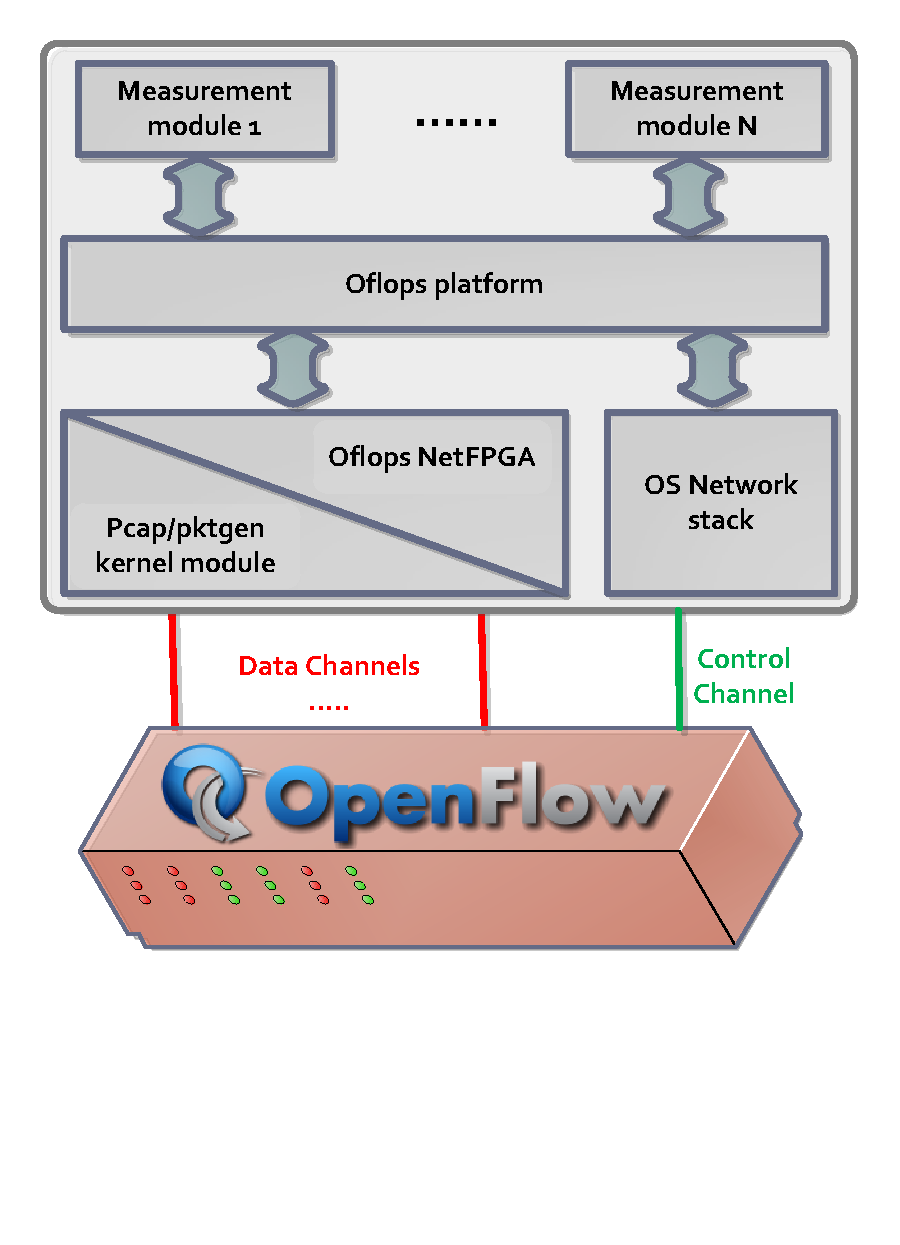
\includegraphics[width=0.9\textwidth]{openflow-design}
\end{center}
\caption{Oflops design schematic}
\label{oflops-design}
\end{figure}

OFLOPS is an OpenFlow testing platform. The main focus of the platform is 
to provide a set of basic measurement test that allow developers to understand and
quantify the capabilities of an OpenFlow enabled device and locate any
possible bottleneck. This platform should be consider as a counterpart of the
oftest platform. The oftest platformcan be used to verify the accurate
implementation of the protocol in terms of semantics, while OFLOPS is focused on the
performance aspect of the implementation. 

In order to assess the performance of a network device that has both
rich functionality and for which we have little idea of the
implementation, we require a diverse set of concurrent measurements
able to encompass all parameters of an experiment. Furthermore,
to achieve high accuracy across a range of control and measurement
tasks, we designed a unified platform that permits us to obtain
information from multiple sources: data and control channels as well
as SNMP to provide specific switch-state information.

A sample design of the platform is
depicted in Figure~\ref{oflops-design}. The platform setups a single control
channel with the switch and uses multiple network ports to generate traffic on
the data plane of the switch. Additionally the platform supports SNMP protocol
in order to read various MIB counters such as CPU utilization, packet counters
etc. 

Some of the features of the platform are the following:
\begin{itemize}
\item Modularity: The platform is split in 2 parts. There is the OFLOPS executable
program which implements the core functionality of the platform and there is a
set of dynamically loaded libraries that implement the required functionality
for a specific test. In order for these two unit to communicate, the platform
defines a rich event-driven API. Each dynamic test can implement a subset of the
provided event handler and adjust the platform behavior to the needs of the
test.
\item Low overhead: The platform focuses to perform multi-level high precision
measurements in order to benchmark the performance of the switch. In order to
achieve minimum delay by the framework, special care has been given to reduce to
a minimum any processing delay. In order to parallelize the processing and
take advantage of modern multicore system, the platform is fully multithreaded.  
\item heterogeneity: The platform provides integration with multiple packet
generation and capturing mechanisms. So far the platform can run both on commodity
PCs with multiport NIC, as well as, NetFPGA equipped systems. Each platform
provides different precision guarantees and costs. 
\end{itemize}

\chapter{Installation}

\section{Source code}

The source code of OFLOPS is available only through git repository.
In order to get a copy of the code, users are required to have installed 
the git command line tools. the source code can be downloaded using the 
following command \footnote{Currently, latest release of the source code is not 
  on the git repo, but user can get an early access view of the code through 
    an e-mail to cr409@cl.cam.ac.uk}: 
    \begin{quote}
    git clone git://gitosis.stanford.edu/oflops.git
    \end{quote}

    In order to build the code, OFLOPS requires two additional git packages. 
    Firstly, it requires the source code of the NetFPGA packet 
    generator c library. Because this library is also stored in a git repository, 
    we have integrate the code as a git submodule and users can download it
    issuing the following command:

    \begin{quote}
    git submodule init \&\& git submodule update
    \end{quote}

    Secondly, users are required to have a version of the OpenFlow header file.
    By default the OFLOPS build configuration expects the OpenFlow reference
    implementation to reside in the directory where OFLOPS code. In order
    for a user to get access to the source code, he can issues the following
    commands:

    \begin{quote}
    git clone git://gitosis.stanford.edu/openflow \\
      git checkout -b release/1.0.0 remotes/origin/release/1.0.0
      \end{quote}

      For the compilation of the OFLOPS code it is required to install a
      series of libraries, namely pcap~\footnote{http://www.tcpdump.org/}, 
      GNU Scientific Library~\footnote{http://www.gnu.org/software/gsl/}, 
      libconfig~\footnote{http://www.hyperrealm.com/libconfig/} 
      and net-snmp~\footnote{http://www.net-snmp.org/} Additionally, if the users 
      require doxygen documentation of the source code, they can get automatically 
      if they install the relevant package. The OFLOPS build configuration script 
      is configured to check for the presence of the 
      doxygen software package and generate the appropriate Makefile if it is 
      present. In the case of a CentOS 5.3 distribution all the required libraries 
      can be installed using the following command.

      \begin{quote}
      yum install gcc automake autoconf libtool libpcap-devel net-snmp-devel
      doxygen gsl-devel\\
        wget http://www.hyperrealm.com/libconfig/libconfig-1.4.7.tar.gz\\
        tar -xvzf libconfig-1.4.7.tar.gz \\
        cd libconfig-1.4.7 \\
        ./configure \\
        make \&\& make install 
        \end{quote}

        In order to build the source code readers must first build the c library of the
        NetFPGA OFLOPS packet generator. Assuming that the user current working 
        directory is the OFLOPS directory, then the following sequence of commands 
        should be issued:

        \begin{quote}
        cd netfpga-packet-generator-c-library/ \\
          ./autogen.sh \&\& ./configure \&\& make \\
          cd .. \\
          ./boot.sh \&\& ./configure \&\& make \\
          \end{quote}

          In case the user wants to use an alternate location for the OpenFlow reference
          implementation, users may use the flag --with-openflow-src-dir= in the
          configuration script and define an alternative location for the default
          \emph{`pwd`/../openflow}. 

          \section{NetFPGA support}

          OFLOPS platform provides integration with the NetFPGA platform.
          We provide together with the OFLOPS source code a binary bitfile of a hardware
          design that enable hardware level packet generation and capturing. 
          Both of these features are
          important for the precision of the measurement, because software packet generation 
          and capture is, on one hand, limited in 
          precision by the OS scheduler and, on the other hand, it is constraint by the 
          bandwidth of the PCI bus. In order to use the hardware extension, the
          user needs to acquire and install a NetFPGA card and its base software system.
          We encourage readers to visit the NetFPGA website for further
          details~\footnote{\url{http://www.netfpga.org}}. Once the NetFPGA platform is
          configure on the host machine, users only need to download the appropriate bitfile to the FPGA
          circuit and modify accordingly the configuration file of OFLOPS. In order to
          download the bitfile, the following command is sufficient. 

          \begin{quote}
          nf2\_download netfpga-packet-generator-c-library/oflops\_packet\_generator.bit
          \end{quote}

          \chapter{Running OFLOPS}

          \section{Introduction}

          OFLOPS builds its testing modules as shared libraries. Modules are 
          loaded at run time using the dlopen functionality of libc. In order to
          configure the test modules loaded during run-time and configure the
          parameters of a test, the OFLOPS tool uses a simple syntax language based on
          the libconfig format. In this chapter we describe the configuration parameter
          that the OFLOPS platform provides.

          \section{OFLOPS configuration files}
          \label{oflops-config-lang}

          The OFLOPS configuration file is based upon the libconfig file syntax, with 
          a strict scheme for the configuration parameters. A set of example configuration 
          files can be found in directory sample\_config/. The OFLOPS configuration file 
          consists of a unique group parameter, named OFLOPS, which contains a set 
          of values that group the configuration parameters based on the generic aspect
          of the functionality that they define. Furthermore, the OFLOPS group contains a 
          scalar parameters that defined which packet generation library will be used. The value is called 
          \emph{traffic\_generation} and has 3 possible values: 
          \begin{itemize}
          \item 1, use userspace packet generator.
          \item 2, user pktgen kenrel generator~\footnote{http://www.linuxfoundation.org/collaborate/workgroups/networking/pktgen}.
          \item 3, use NetFPGA-based packet generator. 
          \end{itemize}
          Regarding the rest of the configuration parameters, they are grouped in 
          the following group parameters: 

          \subsection{control channel configuration}
          For the control section of the configuration file OFLOPS parses the following parameter:
          \begin{itemize}
          \item \emph{control\_dev}: The name of the network device used for the control channel of 
          the controller. This device shouldn't be used at the same time as a data channel. 
          \item \emph{control\_port}: The TCP port on which the OFLOPS controller will listen on.
          \item \emph{snmp\_addr}: The IP address of the SNMP server of the OpenFlow switch.
          \item \emph{cpu\_mib}: A list of MIB entries for the CPU cores of the switch, semicolon 
          separated.
          \item \emph{in\_mib}: The MIB entry of the packet counter of the input queue of the control 
          channel switch port. 
          \item \emph{out\_mib}: The MIB entry of the packet counter of the output queue of the control 
          channel switch port.
          \end{itemize} 

          \subsection{data channel configuration}

          In order to configure the data channels used by an experiment, OFLOPS 
          configuration file contains an array parameter called data which consist 
          of variable number device description. The described network device will
          be used by the OFLOPS testing module in order to generate traffic on the data
          plane of the switch. 

          \begin{itemize}
          \item \emph{dev}: The name of the network device used by the channel. Each 
          network device can only be used once per experiment. 
          \item \emph{port\_num}: The ID of the port of the OpenFlow switch to which 
          the network device is connected. This is required so that the testing modules
          will know which port ID to use on a flow modification message. 
          \item \emph{in\_snmp\_mib}: The SNMP MIB entry for the packet counter of the 
          input queue of the switch port. 
          \item \emph{out\_snmp\_mib}: The SNMP MIB entry for the packet counter of the
          output queue of the switch port. 
          \item \emph{type}: The library used to capture packets over the specific data
          channel. The possible values are \emph{nf2}, for NetFPGA packet capturing, and 
          \emph{pcap}, for libpcap-based packet capturing. 
          \end{itemize}

          \subsection{module configuration}

          Finally the configuration file contains an entry with a variable number
          of module configuration entries. The module entries can be used to locate 
          and initialize appropriately a testing module. Specifically, for each entry
          OFLOPS accepts the following parameters. 

          \begin{itemize}
          \item \emph{path}: The path for the loadable library of the module. 
          \item \emph{param}: A space separate array of module parameters with their 
          respective value. The list of parameters is specific for each module and is 
          described in a great extend in Chapter~\ref{oflops-modules}
          \end{itemize}

          \subsection{Example configuration script}

          In order to provide an example of an OFLOPS configuration file we present the
          following configuration script. In this script we configure the control channel
          to use the device eth1 and open a tcp socket on port 6633, while it will query
          the snmp server on IP 192.168.1.2 in order get feedback from the switch. In this
          experiment we are configuring also two data channels on device nf2c0 and nf2c1
          on which we will be using the the netfpga packet capturing functionality.
          Finally, for the experiment we dictate the OFLOPS to load the shared library
          file libopenflow\_action\_delay.so, to which we pass a series of parameters. 

          \lstset{language=Java,numbers=left,frame=single,title=oflops.cfg}
          \begin{lstlisting}[frame=single]                % Start your code-block
          oflops: {
control: {
           control_dev = "eth1";
           control_port = 6633;
           snmp_addr = "192.168.1.2";
           cpu_mib="1.3.6.1.2.1.25.3.3.1.2.768;1.3.6.1.2.1.25.3.3.1.2.769";  
           in_mib="1.3.6.1.2.1.2.2.1.11.2";
           out_mib="1.3.6.1.2.1.2.2.1.17.2";
           snmp_community = "public";
         };

         data = ({
             dev="nf2c0";
             port_num=1;
             in_snmp_mib="1.3.6.1.2.1.2.2.1.11.3";
             out_snmp_mib="1.3.6.1.2.1.2.2.1.17.3";
             type="nf2";
             },{
             dev="nf2c1";
             port_num=2;
             in_snmp_mib="1.3.6.1.2.1.2.2.1.11.4";
             out_snmp_mib="1.3.6.1.2.1.2.2.1.17.4";
             type="nf2";
             });

         traffic_generator = 3;
         dump_control_channel=0;


module: ({
         path="libopenflow_action_delay.so";
         param="flows=10 data_rate=10 pkt_size=150 ";
         });
          };


\end{lstlisting}

% 
% \section{OFLOPS h/w design}
% \label{oflops-hw}
% 
% The OFLOPS hw design is based on the Stanford Packet Generator design. Using this design as reference we 
% extend some of the functionality, in order to cover the needs of our design.
% Specifically, the desing changes that we performed are the following: 
% 
% Reader should be aware, that the h/w design developed as part of the OFLOPS tool has 

\chapter{OFLOPS Modules}
\label{oflops-modules}

\section{Introduction}

In this section we will provide an in depth description of the testing module
that we have developed  so far using the OFLOPS platform. For each module we describe
the scenario it implements, the configuration parameters that it provides and
its output information. 

\section{openflow\_action\_delay}        

This module is developed in order to measure the impact of the implementation 
of an action on the data plane of a switch. It has been observed in 
some OpenFlow implementation that some of the actions cannot be applied at 
line rate or they are not implemented at all. In order to test the switching
performance of an action, the module initialized the switch flow table with a
single flow that simply outputs packet to a specific output port. This action is
kept in the cache for one minute, while the module generate matching traffic and
measures the switching delay. After one minute the module sends a flow
modification that adds on the action list of the flow a set of user defined
actions, and modifies the output port while it continues to measure the switching 
delay incurred by the switch. By comparing how the number between the two
phases, users can understand whether the action is implemented at line rate and
whether the action incurs any significant delay. 

The module provide the following set of parameters that the user can define:
\begin{itemize}
\item emph{pkt\_size}: This parameter can be used to control the length of
packets of the measurement probe, measured in bytes. Thus, together with the 
  rate parameter, it allows indirectly to adjust the packet throughput of the 
experiment. (default 1500 bytes)
  \item \emph{data\_rate}: The rate of the measurement probe measured in Mbps.
(default 10Mbps) 
  \item \emph{table}: The parameter define whether the inserted flow will be 
a wildcard(value of 1) or exact match(value of 0).  (default 1)
  \item \emph{action}:  A comma separate string of entries of the format
  action\_id/action\_value. E.g. a value of `b/1010,0/2` defines that the action
  will modify the tcp/udp port of the matching packet to a value of 1010 and the
packet will be output on port 2. (default no action)
  \end{itemize}

  The module provide output for the result of the experiment on the log file. 
  Specifically, it outputs 2 lines, one for each experiment phase, with the average, median 
  and variance of the RTT delay of the probe and the packet
  loss, calculated through SNMP. 

  \section{openflow\_flow\_stats \& openflow\_aggr\_flow\_stats}

  These modules are used to understand the possible impact of the flow stats
  extraction functionality of the OpenFlow protocol on the control and data plane of the
  switch. The two modules follow a similar experimental setup, but they differ on
  the type of the flow stat requests that they send. The first module uses the
  flow\_stats\_request OpenFlow message type, while the latter uses the
  aggr\_flow\_stats\_request. 
  The scenario for this experiment is as follows: the flow table is
  initialized with a set of flows for which OFLOPS generates relevant traffic. 
  The measurement traffic consists of 2 probes: a \emph{constant probe}, that
  matches a single flow, and a \emph{variable probe}, that uses at
  random any of the inserted flows. The experiment runs for 1 minute and at 
  the same time the controller queries the switch for its flow statistics over 
  specific intervals. The module stores statistics for the measurement probe, as
  well as, the reply time for the flow statistics and the CPU utilization. 

  The module provides the following configuration parameters:
  \begin{itemize}
  \item \emph{flows}: The total number of unique flow that the module will
initialize the flow table of the switch. (default 128)
  \item \emph{query}: The number of unique flows that the module will query the 
  switch in each flow request. Because the matching method of the module is based 
on the netmask field of the matching field. (default 128)
  \item \emph{pkt\_size}:  This parameter can be used to control the length of the
  packets of the measurement probe. It allows indirectly to adjust the packet
  throughput of the experiment.
  \item \emph{data\_rate}: The rate, in Mbps, of the variable probe. (default
      10Mbps)
\item \emph{probe\_rate}: The rate, in Mbps, of the constant probe. (default 10Mbps)
  \item \emph{query\_delay}: The delay, in microseconds, between the different 
stats requests. (default 10000 usec) 
  \item \emph{print}: A parameter that defines whether the module will output full
  per packet details of the measurement probes. If this value is set to 1, then
  the module will print on a file called "measure.log" for each capture packet a
  comma separated record with the timestamps of the generation and capture times of the
  packet, the packet id, the port at which the packet was captured and the flow id 
of the flow that was used in order to switch the packet. (default 0)
  \item \emph{table}: This parameter controls whether the inserted flow will be
a wildcard(value of 1) or exact match(value of 0). (default 0)
  \end{itemize}

  The output of the module is printed in the log file. The module prints, after the
  end of the experiment, a log line for each flow\_stat\_reply containing timing
  information. Additionally, the module prints RTT and loss statistics for each
  measurement probe. Finally, the module queries the switch every 10 seconds and
  outputs CPU information in the log file. 

  As a future development of this module we are considering the potentiality to
  estimate the accuracy of the statistic extraction mechanism. Unfortunately
  though, so far we are unable to synchronize accurately the result of packet
  counters of the capturing library, with the results of flow\_stats\_reply 
  packets. 

  \section{openflow\_packet\_out}

  This module is developed to measure the performance of the packet\_out
  functionality of the OpenFlow protocol. This message type, allows a
  controller to inject packets in the network by explicitly sending the packet
  data to the switch and defining the output port of the packet. The module
  provide basic measurement on the performance of the OpenFlow implementation
  given a set of parameters. During the experiment, a constant flow of packet\_out
  message is sent to the switch over
  the control channel while the module capture output packets on the data plane of the
  switch. This way the module can calculate the processing delay incurred to such
  message types, as well as, any implication that may occur when the controller
  increases it's sending rate. 

  The module provides the following configuration parameters:
  \begin{itemize}
  \item \emph{pkt\_size}:  This parameter can be used to control the length of the
  packets of the packet\_out message in bytes. It allows indirectly to adjust the packet
throughput of the experiment. (default 1500 bytes)
  \item \emph{probe\_snd\_interval}: This parameter controls the data rate of the 
measurement probe, in Mbps. (default 10Mbps)
  \item \emph{print}: This parameter enables the measurement module to print
  extended per packet measurement information. The information is printed in log
file. (default 0)
  \end{itemize}

  The module outputs in the log file of the program SNMP information from the switch, queried
  every 10 seconds, as well as statistics for the RTT and packet loss of the
  packets inserted using the packet\_out message type. If the parameter 1 is set
  to one, then the module will additionally print per packet timestamps. 

  \section{openflow\_packet\_in}

  This module is developed to measure the performance of the packet\_in
  functionality of the OpenFlow protocol. This message type is generated when a
  packet is received by the switch, that does not match any flow in the flow
  table. For this experiment, the module initially removes any flows in the flow table and starts
  to generate traffic at a specific rate on one of the ports of the switch. 
  In parallel, the module receive packet\_in messages and computer per packet the
  processing delay.

  The module provides the following configuration parameters:
  \begin{itemize}
  \item \emph{pkt\_size}:  This parameter can be used to control the length of the
  packets of the measurement probe. It allows indirectly to adjust the packet
throughput of the experiment. (default 1500 bytes)
  \item \emph{probe\_snd\_interval}: This parameter controls the data rate of the
measurement probe, in Mbps. (default 10Mbps)
  \item \emph{print}: This parameter defines if the measurement module prints
  extended per packet measurement information. The information is printed in log
  file. 
  \end{itemize}

  The module outputs in the OFLOPS log file SNMP information from the 
  switch, queried every 10 seconds, as well as statistics for the RTT and packet 
  loss of the measurement probe, as measured through the packet\_in messages.

  \section{openflow\_reactive}

  This module can be used to understand the scalability properties, when an
  OpenFlow switch is used in a reactive way, similar to the functionality that the NOX
  controller provides. In this case, the controller inserts flows only when a
  packet\_in event is generated. In order to simulate a usage scenario like 
  this, the module initially removes any flows from the switch flow table and starts to generate
  measurement traffic. The measurement traffic matches a specific number of
  exact match flows and packets are generate in a way that matching flows are
  used sequentially. The module logs for each flow the time it received the first
  packet, the time it received the packet\_in message and the time a packet of the
  flow was received on the data plane. 

  The module exports the following parameters:
  \begin{itemize}
  \item \emph{pkt\_size}: This parameter can be used to control the length of the
  packets of the measurement probe. It allows indirectly to adjust the packet
  throughput of the experiment. The parameter uses bytes as measurement unit.
  \item \emph{probe\_rate}: The rate of the measurement probe, measured in Mbps. 
  \item \emph{flows}: The number of unique flows that the measurement flows will
  generate.
  \item \emph{print}:  This parameter enables the measurement module to print
  extended per flow measurement information. The information is printed in log
  file.
  \end{itemize}

  The module outputs in the OFLOPS log file the total delay incurred in order to
  setup all of the flows of the experiment. In addition, the module polls the 
  switch for SNMP packet counters and CPU usage every 10 sec and when the experiment 
  completes and save the query result in the log file. Finally, if the print 
  parameter is enabled, the module output in a CVS files a set of 
  records,  one for each flow, that contain: the flow id and the timestamps of the time the first
  packet of the flow was generated, the time when the first packet\_in event of
  the flow was received by the controller and the time the first packet of the
  received on the data plane. 

  \section{openflow\_add\_flow  \& openflow\_mod\_flow}

  This set of modules can be used to measure the scalability properties of the flow
  table. The modules measure the delay that the switch incurs when the controller
  modifies the content of the flow table. The difference between the two modules is that the first
  module considers only flows insertions, while the later focuses on flow updates.
  The experimental scenario works as follows: During the initialization of the
  experiment a set of flows is inserted in the flow table in order to switch all
  of the traffic in the data plane. For the case of flow additions, the module
  insert a single wildcarded flow that outputs data to port 3 of the 
  experiment, while for flow modification, the module inserts a number of flows in the flow
  table equal to the number of flows in the data plane that output matching
  packets to port 3. The measurement traffic consists of 2 probes: a \emph{constant probe}, that
  matches a single parameter, and a \emph{sequential probe}, that uses in a round
  Robbin manner all of the inserted flows. We use two measurement probes
  because we are interested to measure the delay to insert both a single flows as
  well all of the flow. The experiment keeps the initial content of the flow table 
  for 30 seconds, in order for the switch to reach a
  steady state, and then sends a series of flow modification and a barrier
  request. The module monitors all ports and stores information of the time 
  when each new flow modification becomes active and when the barrier reply is
  received. 

  The module provides the following configuration parameters: 
  \begin{itemize}
  \item \emph{pkt\_size}: This parameter can be used to control the length of the
  packets of the measurement probe. It allows indirectly to adjust the packet
  throughput of the experiment. The parameter uses bytes as measurement unit.
  The parameter applies for both measurement probes. 
  \item \emph{probe\_rate}: The rate of the sequential probe, measured in Mbps. 
  \item \emph{data\_rate}: The rate of the constant probe, measured in Mbps. 
  \item \emph{flows}:  The number of unique flows that the module will
  update/insert.
  \item \emph{table}:  This parameter controls whether the inserted flow will be
  a wildcard(value of 1) or exact match(value of 0). For the wildcard flows, the
  module wildcards all of the fields except the destination IP address. 
  \item \emph{print}: This parameter enables the measurement module to print
  extended per packet measurement information. The information is printed in a
  separate CSV file, named "action\_aggregate.log".
  \end{itemize}

  The module logs in the OFLOPS log file the timestamps when the flow
  modification and barrier request transmission starts(entry label:
      START\_FLOW\_MOD, BARRIER\_REPLY) 
  and ends(entry label: END\_FLOW\_MOD) and when each flow becomes active in the data 
  plane(entry label: FLOW\_INSERTED). Additionally, the module prints for each
  channel statistics regarding the RTT and packet loss for each data channel. 

  \section{openflow\_echo\_delay}

  This module can be used to measure the processing delay of the control channel.
  Specifically, it generated echo\_request messages for one minute, and calculates the delay
  for the switch to reply. The module provides a single configuration 
  parameter, \emph{delay}, which define the inter-request delay in microseconds. 

  The module outputs in the log file a line for each echo\_reply, that
  contains all the required timing information, for offline analysis. The
  module also output at the end of the measurement an entry with mean, median and
  variance of the reply delay as well as any possible reply loss. 

  \section{openflow\_interaction\_test}

  This test was developed in order to understand how the flow stats extraction
  mechanism may interfere with other control plane operations. In this experiment
  we repeat the scenario described in the openflow\_flow\_stats module, but
  after 1 minute the module tries to modify the flow table of the switch. In
  parallel the module monitors the time it takes for the new flows to become
  active on the data plane. 

  The module exports the following configuration parameters:
  \begin{itemize}
  \item \emph{pkt\_size}: This parameter can be used to control the length of the
  packets of the measurement probe. It allows indirectly to adjust the packet
  throughput of the experiment. The parameter uses bytes as measurement unit.
  The parameter applies for both measurement probes.
  \item \emph{probe\_rate}: The rate of the sequential probe, measured in
  Mbps.
  \item \emph{data\_rate}: The rate of the constant probe, measured in Mbps.
  \item \emph{flows}:  The number of unique flows that the module will
  update/insert.
  \item \emph{table}:  This parameter controls whether the inserted flow will
  be
  a wildcard(value of 1) or exact match(value of 0). For the wildcard 
  flows, the module wildcards all of the fields except the destination IP address.
  \end{itemize}

  The module will output on the OFLOPS log file, all the details described in the
  openflow\_flow\_stats and openflow\_add\_flow modules. 

  \section{openflow\_timer}

  With this measurement module, users can quantify the precision of the internal
  timers of an OpenFlow switch. The OpenFlow protocol, provides for each flow a
  couple of parameters that allows the controller the time for which a flow will be
  effective. Once the timers have expired, the switch is obliged to remove the
  flow from the flow table and inform the controller with an appropriate 
  message, if the flow has a specific flag set. In this experiment, the flow table is
  initialized with a default flow with low priority that switches packets to port
  2 and in parallel it generate a sequential measurement probe that match a specific
  range of flows. After a second of experimental run time, the controller insert a
  set of new high priority flows that match the packets of the measurement probe 
  and output packets to port 3 of the switch. Each flow has a specific hard timeout 
  value assigned to it as well as the OFPFF\_SEND\_FLOW\_REM flag set. The module monitors 
  the duration that the flows are active, using the data plane of the switch, as 
  well as the duration feedback that it receives from the FLOW\_REM message and
  stores them in the log file of OFLOPS. 

  The module provides the following configuration parameters:
  \begin{itemize}
  \item \emph{pkt\_size}: This parameter can be used to control the length of the
  packets of the measurement probe. It allows indirectly to adjust the packet
  throughput of the experiment. The parameter uses bytes as measurement unit.
  The parameter applies for both measurement probes.
  \item \emph{data\_rate}: The rate of the constant probe, measured in Mbps.
  \item \emph{flows}:  The number of unique flows that the module will
  update.
  \end{itemize}

  \section{snmp\_queue\_delay}

  This module is developed in order to measure the switching performance in the
  data plane of the switch. This test is important mostly for software
  switches, as hardware switches perform switching at line rate using
  specialized hardware designs resulting in negligible processing delay. 
  In this experiment the module initializes the flow table with a single
  flow that output packets to a specific port. The module generates traffic at
  various rates for a specific time period and measure for each packet the switching delay. 
  Specifically, the module tests for data rates of 1, 10, 64, 128, 256, 512 and 1000 Mbps.

  The module accepts the following configuration parameters:
  \begin{itemize}
  \item \emph{pkt\_size}: This parameter can be used to control the length of the
  packets of the measurement probe. It allows indirectly to adjust the packet
  throughput of the experiment. The parameter uses bytes as measurement unit.
  \item \emph{duration}: The duration of the measurement period for each probing
  rate. The measurement unit is seconds and the default value is 30. 
  \end{itemize}

  The module will output in the OFLOPS log a set of records which provide for each
  probing rate the mean, median and variance of the RTT and the packet loss. 

  \section{snmp\_tuple\_test}

  In this module we are testing all possible combinations of the OpenFlow toppled in
  order to quantify any possible the impact of the tupple format to the data plane. This test
  design occurred by the fact that some of the early implementations, did not
  support at full extend the OpenFlow tupple. The module uses a single flow entry
  and a single flow measurement probe. For each possible tupple combination the
  controller send a flow modification with the appropriate flow match and then
  sends traffic for a specific period of time. For each test, the module stores in the
  log file the RTT and loss statistics of the flow. 

  The module provides two possible parameters for this module: \emph{pkt\_size}
  and \emph{duration}. The pkt\_size controls the length of the packet of the
  measurement probe. The duration is used to define to the module the duration of
  each tupple test. Currently the default value is 10 seconds. The module
  outputs on the OFLOPS log file for each match case a line with statistics for
  the RTT and packet loss of the measurement probe.  
  
  \section{openflow\_dummy}

  This module is a simple reference module that is included in order to exemplify
  to user all the potential API calls that a module can implement. This module
  does not implement any functionality and should not be used in any test.

  %\section{oflops\_debug}
  %
  %\section{openflow\_action\_measurement}
  %
  %A module to measure the delay for a switch to reply to 
  %
  %\section{openflow\_flow\_dump\_test}
  %\section{openflow\_port\_status}
  %\section{openflow\_vlan\_mod}
  %\section{snmp\_cpu}
  %\section{openflow\_action\_install}
  %\section{openflow\_path\_delay}

  \chapter{Developing OFLOPS modules}

\section{OFLOPS API design}
\section{Module life-cycle}
\section{OFLOPS Events}
\subsection{Timer Events}
\subsection{Control Channel Events}
\subsection{Data Channel Events}
\subsection{SNMP events}

  \end{document}
